\chapter{Design}

The architectural design of MCDTP uses both TCP and UDP connections. Like \cite{Meiss2007}, \cite{He2002}, \cite{Aspera2016}, and \cite{Fan2010}, MCDTP uses the UDP transport protocol for the data transfer and the TCP socket is used for exchanging messages between the server and client. The experimental component of this protocol is the lack of congestion control. As mentioned here, \cite{Aspera2016} \cite{Fan2010}, the observed bottleneck resides on the hosts of an end-to-end transfer. MCDTP seeks to mitigate this through multiple asynchronous data channels and the number of channels is based on the degree of parallelism of the host machine. A channel acts as a pipe from disk to socket and vice versa. This is how MCDTP tries to provide continuous data flow. As a disclaimer, the term ``packet(s)" hereinafter does not refer to Transport or Network layer packets, the term is used to refer to an Application layer structure used by MCDTP.

\section{Protocol Design}

The MCDTP protocol focuses on being a very simple and lean protocol to try and minimize the needed time to process incoming messages or data. The protocol consists of three phases: a double handshake phase, data transmission phase, and retransmission phase. For TCP communication, each packet consists of 15 bytes. Each packet is a header with an optional payload. All headers begin with two fields, ``ptype" and ``subtype". These two fields specify how the packet should be processed. The UDP packet is adjustable in size when implementing MCDTP. It is, however, required to be within the following scope: $13B < size < 64KB$. The 13 byte lower bound is to account for packet header. The 64 kilobyte upper bound can be found here \cite{postel1981ip}. Unlike the TCP packets, UDP packets include payload size with packet size. Since TCP has the option of a payload, when one exists, a second read from the stream will be required to grab the payload. With the UDP packet, it is guaranteed that a packet will be a set size and thus eliminates the need for a second read.

\subsection{Two Step Handshake}

As with many protocols, MCDTP has a handshake step. However, MCDTP performs two handshakes, the first upon connection and the second before a data transfer. The purpose for the two step handshake is for the sake of extensibility, i.e. another step or function could take place between both handshakes.

\subsubsection{Specification Handshake}

The specification handshake occurs when a client connects to the server. Figure \ref{fig:specs} illustrates the type of communication that happens during the handshake.

\begin{figure}[ht]
\centering
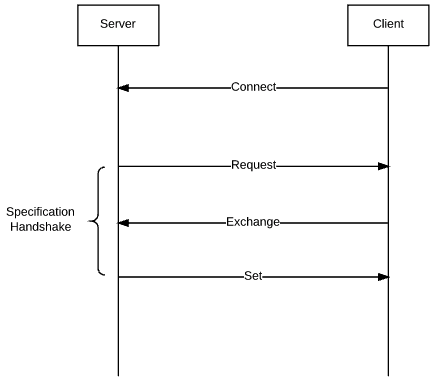
\includegraphics[scale=0.7]{SpecificationHandshake}
\caption{Illustration of Specification Handshake}
\label{fig:specs}
\end{figure}

The purpose of this handshake is ensure that both client and server use the same specifications for a data transfer. These specifications currently include the exchange and selection of ports the client should use for each UDP socket. As a side effect, the server knows the degree of parallelism of the client and can also effect this aspect as well based on how many ports it selects. The degree of parallelism for both hosts is set to whichever machine has the smaller degree of parallelism. In the instance of mismatch, there will be a machine whose potential is under utilized. This option is preferred over the other possible options such as increasing the degree of parallelism of the smaller machine to match the larger machine, or allowing them to be mismatch. The outcome of increasing the degree of parallelism would result in the smaller machine working too hard and ultimately slowing down due to the excess number of context switches being performed. If the latter alternative was in the scenario where the server was the larger machine and the client was the smaller machine, any implementation of MCDTP would then either force more than one UDP socket on the server to be mapped to one UDP socket on the client resulting in that socket being flooded with too much data, or, a server UDP socket would be idle and thus resources would be wasted. If the roles were reversed, the client would have an idle socket. The optimal choice is reducing the degree of parallelism to match.

\begin{figure}[ht]
\centering
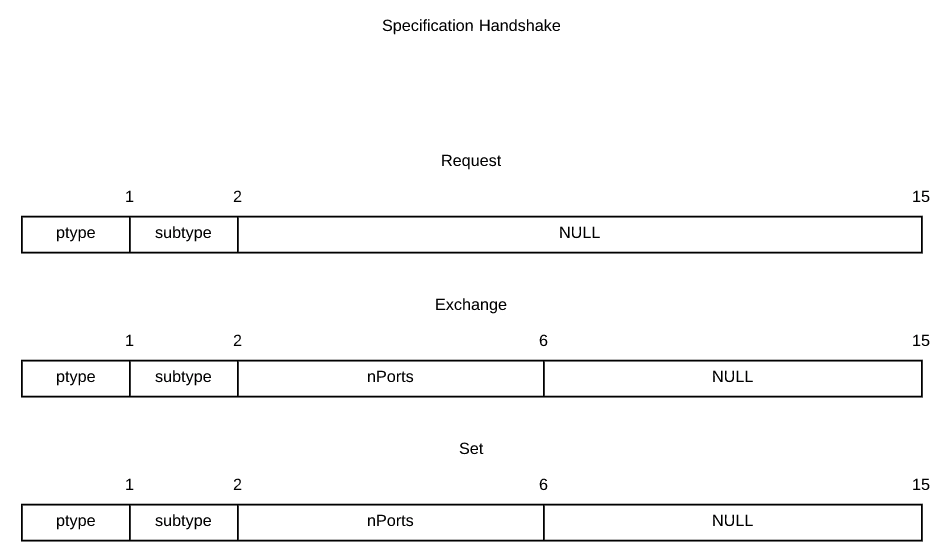
\includegraphics[scale=0.4]{SpecificationHandshakePacketStructures}
\caption{Packet Structure of Specification Handshake}
\label{fig:specs-struct}
\end{figure}

Figure \ref{fig:specs-struct} shows the packet structure of each message, excluding connect, in the handshake. The value of ``ptype" and ``subtype" are as follow for each packet: $Request \rightarrow ptype = \lq{s}\rq,subtype = \lq{r}\rq$, $Exchange \rightarrow ptype = \lq{s}\rq,subtype = \lq{N}\rq$, $Set \rightarrow ptype = \lq{s}\rq,subtype = \lq{n}\rq$. In this handshake, both Exchange and Set have an additional field, ``nPort", and are followed by a payload. The payload consists of port values, which ``nPort" specifies how many port values are in the payload. In order to be as language agnostic as possible, a port is represented as 4 bytes, or a 32bit integer. Given this, the payload size can be calculated so that an exact number of bytes can be read during the second read from stream.

\subsubsection{FTP Handshake}

Prior to transferring a file, MCDTP performs another handshake that is similar in design, as can be seen in Figure \ref{fig:ftp-hs}.

\begin{figure}[ht]
\centering
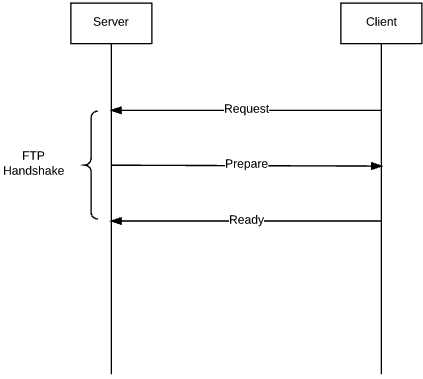
\includegraphics[scale=0.7]{FTPHandshake}
\caption{Illustration of FTP Handshake}
\label{fig:ftp-hs}
\end{figure}

This handshake acts as a concrete step before the data transmission phase and is very simple in design and purpose. This step is so that any asynchronous work that needs to be done first can finish as well as making sure both client and server are prepared for the data transmission phase, which mostly involves Disk I/O preprocessing steps, more on this in section \ref{sec:disk-io}. Figure \ref{fig:ftp-struct} is an illustration of the structure of each message in the handshake.

\begin{figure}[ht]
\centering
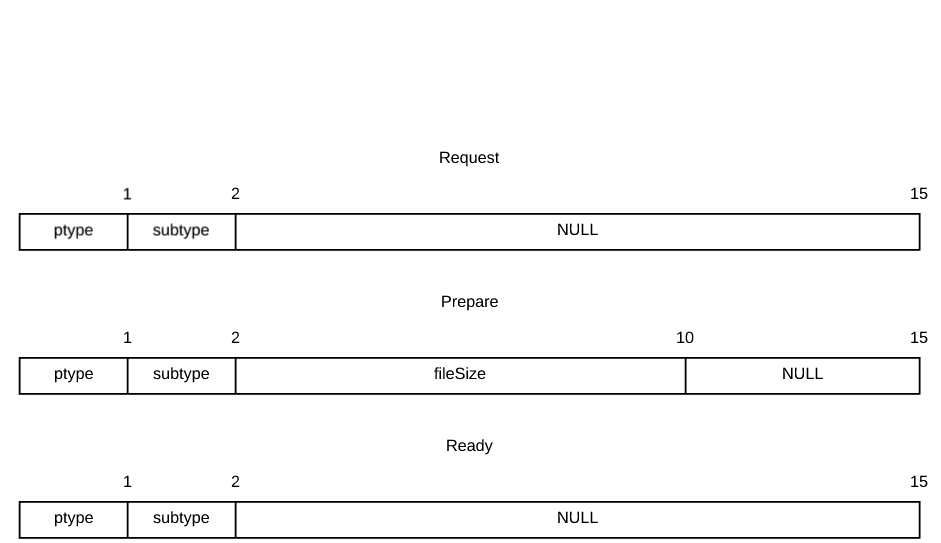
\includegraphics[scale=0.4]{FTPHandshakePacketStructures}
\caption{Packet Structure of FTP Handshake}
\label{fig:ftp-struct}
\end{figure}

 The value of ``ptype" and ``subtype" are as follow for each packet: $Request \rightarrow ptype = \lq{t}\rq,subtype = \lq{r}\rq$, $Prepare \rightarrow ptype = \lq{t}\rq,subtype = \lq{p}\rq$, $Ready \rightarrow ptype = \lq{t}\rq,subtype = \lq{R}\rq$. The only information exchanged in this handshake is the size of the file that will be transferred, from server to client. Note that handling file selection has been omitted and will be further discussed in chapter \ref{chp:c-fw}. Once the client is prepared for transfer and has signaled the server that it is ready, both hosts begin the data transmission phase of the MCDTP protocol.

\subsection{Data Transmission}

<Add text>

\subsection{Packet Retransmission}

<Add text>

\section{Disk I/O}\label{sec:disk-io}

<Add text>

\subsection{File Partitioning}

<Add text>